\title{SMU – Bayesovká síť}
\author{Lukáš Hromadník}
\maketitle

\section{Baseline model}

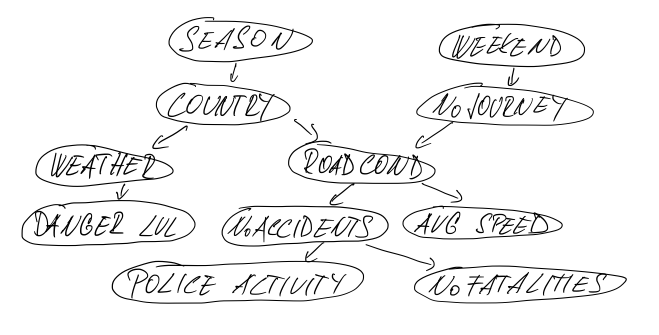
\includegraphics[width=0.75\textwidth]{sit.png}

\section{Závislosti}

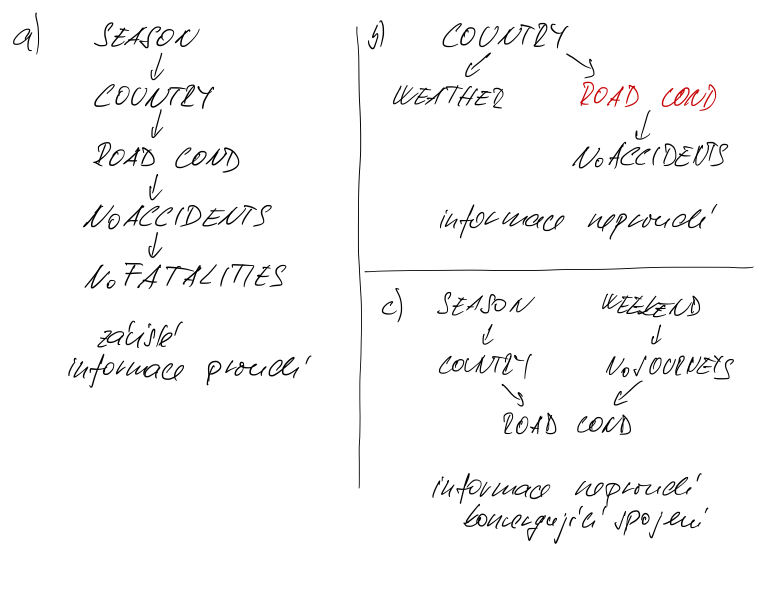
\includegraphics[width=0.75\textwidth]{independence.png}

\section{Interpretace CPT}

\begin{tabular}{| l | l | l | l | l | l | l |}
\hline
Country & Europe & Europe & UK & UK & US & US \\ \hline
NoJourneys & Low & Medium & Low & Medium & Low & Medium \\ \hline
RoadCond(bad) & 0.66 & 0.39 & 0.63 & 0.44 & 0.62 & 0.39 \\ \hline
RoadCond(good) & 0.34 & 0.61 & 0.37 & 0.56 & 0.39 & 0.61 \\ \hline
\end{tabular}

Pokud se po silnici jezdí více aut, potom je silnice s větší pravděpodobností v lepší kondici. Naopak pokud se po silnici jezdí málo, tak je ve špatném stavu.

\section{Odvození finálního modelu}

Finální model byl odvozen pomocí metody Hill Climbing.